\documentclass[12pt]{article}
\usepackage[francais]{babel}
\usepackage[UTF8]{inputenc}
\usepackage[T1]{fontenc}
\usepackage{times}
\usepackage{helvet}
\usepackage{graphicx}
\usepackage{fancyhdr}
\usepackage{eurosym}
\usepackage{color}
\usepackage{soul}
\usepackage[ left = 4.5cm, right = 3.5cm]{geometry}


\renewcommand{\baselinestretch}{1.5}
\setlength{\parindent}{3cm}

\pagestyle{fancyplain} \chead{}\lhead{\textit{Les Professionnels}} \rhead{\emph{\textit{Evasion}}}

\definecolor{pseudorouge}{RGB}{200, 50, 50}
\definecolor{pseudoblue}{RGB}{20,10,230}
\definecolor{texteGris}{RGB}{50,50,75}

\begin{document}
\thispagestyle{empty}
\begin{center}
\fontsize{21}{21}{\textbf{Rapport de Soutenance 2 \vspace*{0.2cm}}}

\end{center}

\vspace*{0.7cm}

\begin{center}
\fontsize{21}{21}{\textbf{- Les Professionnels/}}
\fontsize{21}{21}{\textbf{2013-2014 -}}
\end{center}

\vspace*{0.5cm}

\begin{center}

\includegraphics[scale=01.0]{evasion}
\end{center}

\vspace*{0.5cm}

\fontsize{14}{14}
\begin{center}
{Lenny \textcolor{pseudorouge}{\textit{"Le Noob"}} Danino - danino\_l}
\end{center}
\begin{center}
Louis \textcolor{pseudoblue}{\textit{"El Parain"}} Kédémos - kedemo\_l
\end{center}
\begin{center}
Anatole \textcolor{pseudoblue}{\textit{"Totonut"}} Moreau - moreau\_a
\end{center}
\begin{center}
Khalis Chalabi - chalab\_k
\end{center}

\begin{center}

\includegraphics[scale=00.20]{infini}
\end{center}


\setlength{\headheight}{13pt} % Haut de page
\setlength{\headsep}{2.5cm} % Entre le haut de page et le texte
\setlength{\footskip}{2.5cm}



\setcounter{tocdepth}{1} 


\newpage
\thispagestyle{empty}
\pagestyle{fancyplain} \chead{}\lhead{\textit{Les Professionnels}} \rhead{\emph{\textit{Evasion}}}
\tableofcontents


\newpage
\section{Khalis Chalabi}
\subsection{Récapitulatif des deux premières soutenances}
\subsubsection{Soutenance 1}
Pour cette première soutenance je devais implémenter plusieurs classes, faire bouger un personnage 3D et je m'étais fixé comme objectif acquérir des bases en développement web pour pouvoir commencer à développer le site de notre jeu vidéo avec l'aide d'Anatole. Au début de l'année mon niveau en programmation n'était pas suffisant pour pouvoir réaliser les tâches que mon groupe m'avait confiées. Mon travail dans ce projet a donc débuté avec un très grand travail de recherche. Les tutoriels et les aides trouvés sur Internet, mais surtout, les membres de mon groupe m'ont permis d'élargir mes connaissances en informatique.


Les TPs réalisés au cours de l'année m'ont permis d'implémenter les classes Personnages, Objets et Décors sans faire plus de recherches. Cependant, faire déplacer un personnage 3D à l'aide du clavier me dépassais complètement. Je me suis donc mis à la recherche d'un tutoriel qui allait pouvoir me permettre de réaliser cet objectif. Le site du Zéro étant un site complet et détaillé pour les débutants, je me suis rendu sur ce site pour commencer. J'ai pu y trouver un tutoriel expliquant le développement de jeu vidéo avec XNA. A première vu ce tutoriel semblait parfait pour moi vu que notre jeu vidéo devait fonctionner sous XNA. Les explications étaient plutôt simples si l'on avait déjà quelques bases en C\# ce qui était mon cas. Le tutoriel débutait avec un rappel de ce qu'était XNA et ce qu'on pouvait faire avec ce Framework. Puis il expliquait l'utilisation des sprites, et pour finir, comment faire interagir une image avec le joueur. Cependant, il est ici question de 2D or notre jeux vidéo est un jeu en 3D. Malgré cela, ce tutoriel m'a grandement aidé pour comprendre comment faire bouger une image avec les touches du clavier ou une souris. J'avais donc enrichi mes connaissances en programmation et pouvais, dorénavant, commencer à essayer de faire bouger mon personnage 3D.

Lors de la 2ème soutenance il est obligatoire de présenter un site web. Un membre de notre groupe, Anatole, possédais déjà les connaissances nécessaires pour la création d'un site web. Cette partie m'intéressais je lui ai donc proposé de nous occuper du site web ensemble. Cependant, encore une fois, mes connaissances étaient légères. Le site du Zéro me fût encore d'une très grande aide car c'est grâce à celui-ci que je pu apprendre les bases de HTML5 et de CSS3 deux langages webs utilisés majoritairement pour la création de site web.

Mes recherches finies, j'essayais de mettre en pratique ce que j'avais appris. Comme je vous l'ai précisé dans les paragraphes précédents, mais sans entrer dans les détails, j'étais chargé d'implémenter les classes Personnages, Objets et Décors. Parmi les tâches qui m'étaient attribuées j'ai décidé de commencer par celle-ci car grâce aux TPs, je savais ce qu'était une classe et comment cela fonctionnait. Cependant il n'y avait pas juste trois classes à implémenter mais beaucoup plus! En effet la classe Personnage était la classe mère et elle possédait des classes filles : la classe Ennemi, la classe Joueur ainsi que la classe PNJ (personnages non jouables). Et il en était de même pour les classe Objets et Décors elles possédaient chacune plusieurs classes filles. La classe mère, Personnages, et ses classes filles furent les plus longues et les plus dures à coder. Elles comportaient plusieurs fonctions et les constructeurs étaient assez longs. Après avoir bien compris la logique les classes Objets et Décors ainsi que leurs classes filles ne furent pas très difficile à implémenter.

Le déplacement du personnage 3D fût la tâche la plus difficile à exécuter vu qu'il fallait interagir avec le joueur et que ce n'était pas une notion que nous avions abordé en TP. Comme je vous l'ai dit précédemment j'ai suivi un tutoriel sur le site du Zéro. Le tutoriel était destiné à un jeu en 2D mais cela ne changeait pas grand-chose au déplacement du personnage en 3D. Il faut juste comprendre qu'en 3D nous utilisons un modèle et qu'en 2D ce sont des sprites. Pour que l'utilisateur puisse contrôler les déplacements du personnage à l'aide du clavier, il suffisait de récupérer l'état du clavier et, en fonction des touches qui sont enfoncés, faire varier la position du personnage 3D ainsi que sa vitesse. Après m'avoir occupé de cette partie il était donc possible de diriger le personnage principal à l'aide des touches directionnelles.

Voici donc, le travail que j'ai fourni pour cette première soutenance. Un travail qui ne fût pas des moindres mais qui m'apporta beaucoup en ce début d'année.

\subsubsection{Soutenance 2}
\par
Nous sommes maintenant à un peu plus du milieu de l'année et mes connaissances ainsi que mon niveau en informatique sont un peu plus développés. Cependant, pour cette deuxième soutenance, il m'a encore fallu mener un travail de recherche. Parmi les tâches qui m'incombait, les graphismes et le mode multijoueur étaient des tâches complexes étant donné que je ne savais pas par où commencer.  

\par
Le graphisme fût une des tâches les plus difficiles à réaliser car il fallait que j'utilise deux logiciels avec lesquels je n'avais jamais travaillé : Photoshop et Blender. Nous faisons un jeu en 3D donc il ne suffisait pas d'importer des sprites et des textures avec XNA comme pour un jeu en 2D. Louis a créé ce qu'on appelle des modèles avec l'aide du logiciel Blender. Ce logiciel permet, entre autre, de modéliser des images en 3D. Nous avions donc la forme principale de nos personnages, il fallait ensuite les personnaliser (lui faire porter des vêtements, lui faire un visage...) Il nous a d'abord fallu découper notre modèle pour obtenir un patron car pour personnaliser le personnage il faut appliquer une texture sur chacune des faces du modèle.
\newline

\newpage

\begin{figure}[t]
\begin{center}
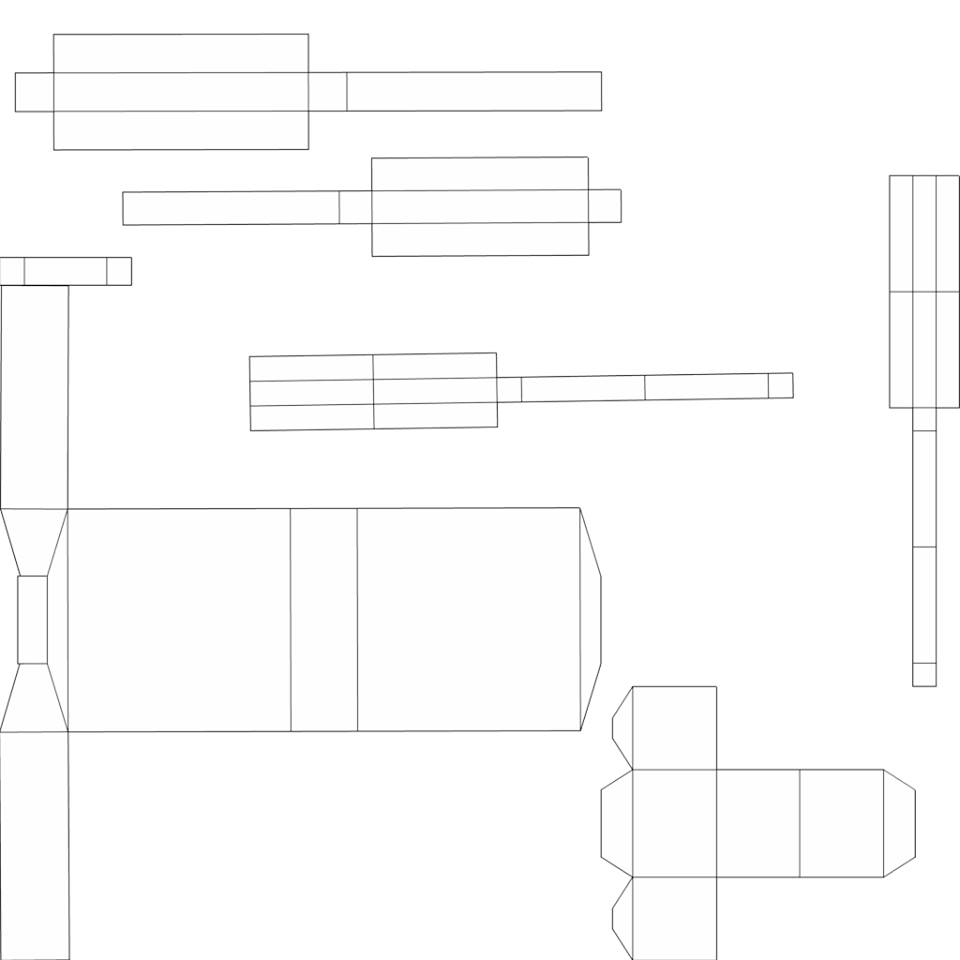
\includegraphics[scale=0.3]{decoupe.jpg}
\caption{Patron du personnage}
\end{center}
\end{figure}


\par
Pour découper notre modèle nous avons utilisé Blender, il fallait découper les faces mais en faisant attention d'en garder une qui soit rattacher aux autres. Imaginez la découpe d'un cube nous a beaucoup aidé. Une fois le modèle complètement découpé nous obtenons l'image ci-dessus. Vous avez peut-être l'impression que cela ne ressemble à pas grand-chose mais en reconstruisant le patron vous obtenez bien le modèle de notre personnage. En haut à gauche de l'image vous avez ses deux bras, juste en dessous et sur la droite ses deux jambes, la plus grosse figure correspond au haut du corps (torse, dos, cou...) et enfin tout en bas à droite sa tête. Une fois ce travail fait il fallait donner l'aspect que nous voulions au personnage. Pour cela j'ai dû utiliser le logiciel Photoshop car pour chaque face du patron il faut comme je vous l'ai dit précédemment une texture. Je me suis occupé de faire le personnage principal ainsi que les gardiens de prison. Je sélectionnais une image qui me plaisait sur Internet puis je prenais la partie qui m'intéressait grâce aux fonctionnalités de Photoshop. Par exemple pour faire le dos du gardien j'ai choisi une image de gardien de prison vu de dos puis j'ai rogné l'image de façon à avoir que le haut de l'uniforme. La difficulté dans cette partie était que je n'avais jamais utilisé Photoshop donc j'ai dû découvrir ce logiciel au fur et à mesure. Lorsque j'avais des problèmes je me renseignais sur Internet ou demandais de l'aide à Louis qui connaît plutôt bien ce logiciel. M'occuper du design des personnages m'a donc demandé beaucoup de temps. Je devais faire de nombreux tests pour obtenir ce que je voulais.
\newline

\begin{figure}[htbp]
\begin{minipage}[c]{.45\linewidth}
\begin{center}
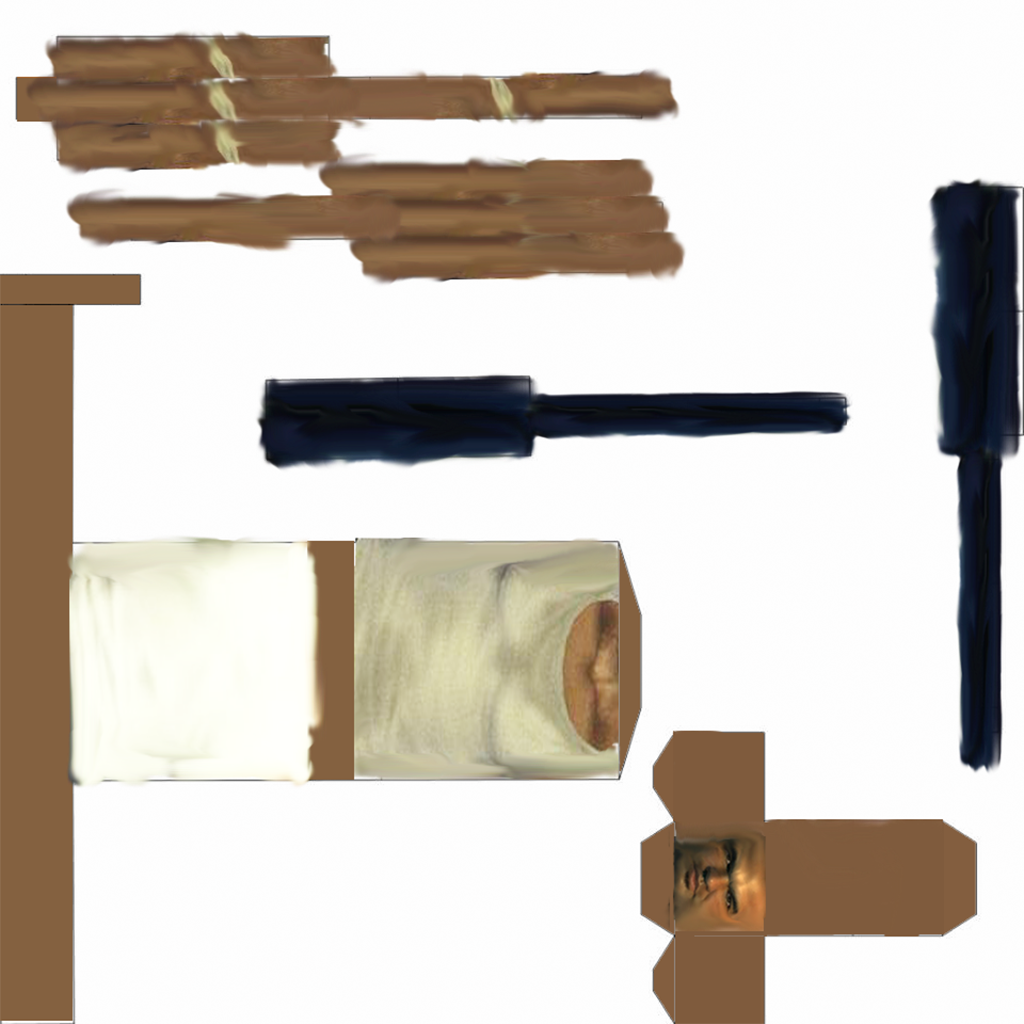
\includegraphics[scale=2]{michaelphotoshop.png}
\caption{Texture personnage principal}
\label{fig:michaelphotoshop}
\end{center}
\end{minipage}
\hfill
\begin{minipage}[c]{.45\linewidth}
\begin{center}
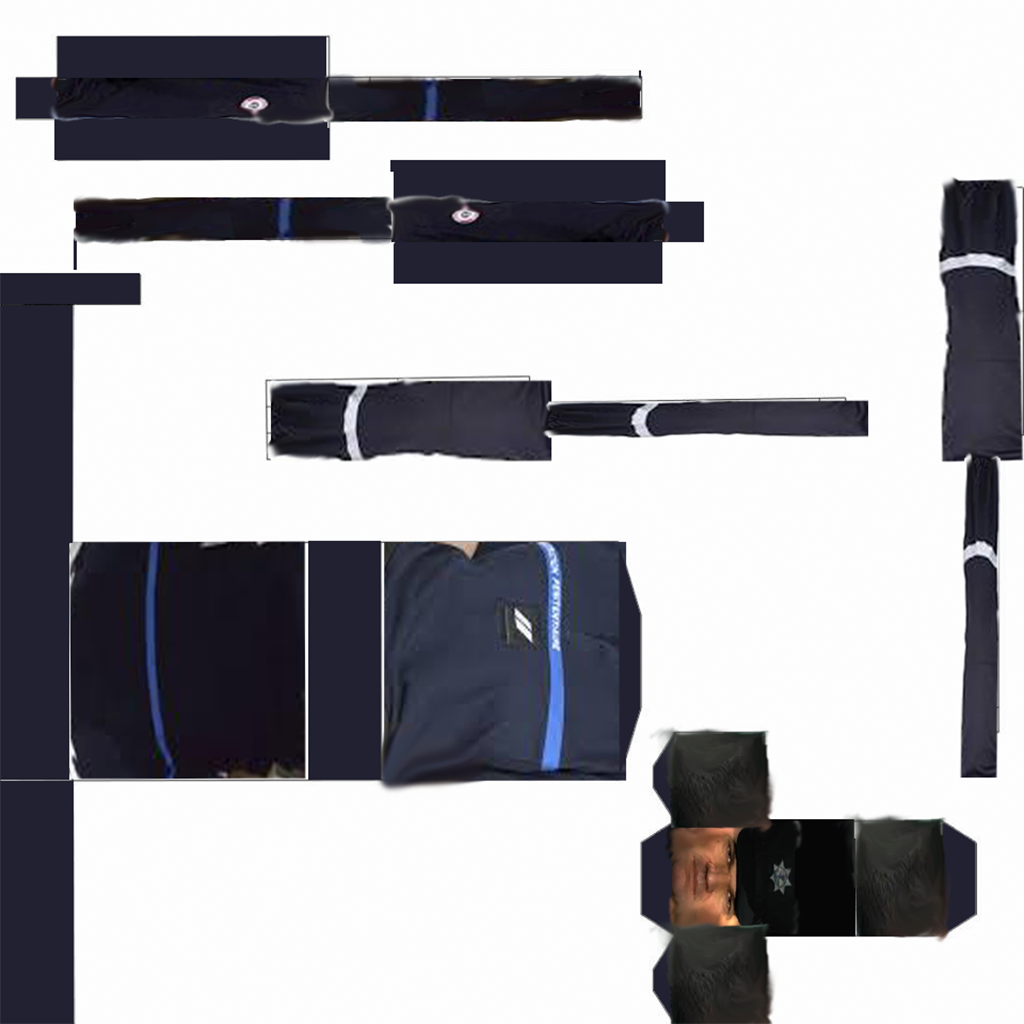
\includegraphics[scale=2]{bellikphotoshop.png}
\caption{Texture gardien de prison}
\label{fig:bellikphotoshop}
\end{center}
\end{minipage}
\end{figure}

\par
Une fois que j'avais fini d'appliquer des textures au patron, j'importais l'image sur Blender pour pouvoir vérifier l'aspect de mon personnage parce qu'avec le patron, comme vous pouvez le voir, on ne s'en rend pas compte. Je regardais l'aspect de mon personnage à chaque modification pour pouvoir éviter de tout recommencer si cela ne me plaisait pas.
\newline

\begin{figure}[htbp]
\begin{minipage}[c]{.45\linewidth}
\begin{center}
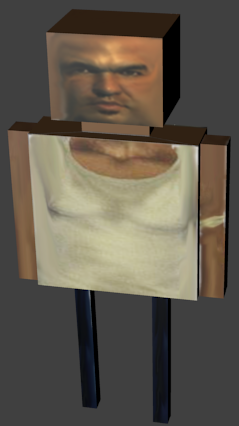
\includegraphics[scale=0.6]{michael.png}
\caption{Personnage principal}
\label{fig:michael}
\end{center}
\end{minipage}
\hfill
\begin{minipage}[c]{.45\linewidth}
\begin{center}
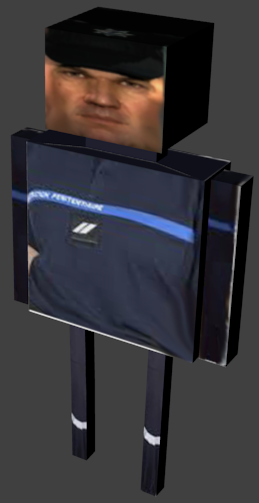
\includegraphics[scale=0.5]{bellik.png}
\caption{Gardien de prison}
\label{fig:bellik}
\end{center}
\end{minipage}
\end{figure}

\par
Une fois le premier personnage fait le deuxième fût plus simple à faire car j'avais pu m'habituer à Photoshop et à Blender. Le plus facile dans cette partie fût la réalisation du mur de la prison. Étant donné qu'en 3D un mur est juste un rectangle le découpage est plutôt simple par rapport au découpage du modèle du personnage. Il suffisait ensuite d'importer l'image d'un mur dans Photoshop puis de légèrement la modifier. Cela nous a donc permis d'avoir les principaux personnages et le début du décor ce qui est une grande avancée car notre jeu vidéo commence enfin à ressembler à un jeu vidéo.

\par
Comme dans la plupart des jeux vidéo, notre personnage possède une barre de vie. Cette dernière se vide en fonction des dégâts reçus et peut se remplir si le personnage se soigne. Elle possède en son centre un nombre qui permet de connaître le nombre de points de vie actuel sur le nombre de points de vie maximum. Pour créer cette barre de vie j'ai implémenté une nouvelle classe nommée ''BarreDeVie''. Avant de commencer à coder, j'ai tout d'abord créé le design de ma barre de
vie à l'aide de Photoshop. J'ai dû créer deux textures : la barre de vie et sa bordure. Une fois cette étape réalisée j'ai pu commencer à implémenter ma classe. Ce ne fut pas très long, la classe ne contenait qu'un constructeur et 4 fonctions. La première fonction me permettait d'ajuster la barre de vie de telle sorte que les points de vie ne soit pas négatifs ou qu'ils ne dépassent pas la valeur maximale définie. Ensuite une fonction qui mettait à jour la barre de vie par rapport au niveau de santé du personnage. Puis pour finir les deux fonctions les plus difficiles. Celle qui permet de réduire la barre de vie normalement et celle qui la dessine dans les bonnes proportions. En effet, lorsque les points de vie diminuaient ou augmentaient la totalité de la barre (le fond rouge ainsi que la bordure) diminuait mais se rapetissait également jusqu'à devenir extrêmement fine et minuscule! De plus elle se dessinait dans de mauvaises proportions car elle prenait toute la longueur de l'écran. Pour régler ces problèmes j'ai utilisé deux surcharges différentes de la fonction ''Draw'' une pour la bordure et l'autre pour le fond. L'affichage du nombre de point de vie est tout simplement possible avec l'utilisation d'un ''SpriteFont''. Pour que tout s'affiche correctement il ne manquait plus qu'à déclarer, initialiser, charger et dessiner la barre de vie dans la classe ''game''.

\begin{figure}[h]
\begin{center}
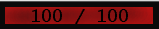
\includegraphics[scale=1.5]{Barredevie.png}
\caption{Barre de vie}
\end{center}
\end{figure}

Un de mes objectifs pour cette deuxième soutenance était de commencer à implémenter un mode multijoueur. Je pense que je m'en suis plutôt bien sorti car il est pratiquement fini (on peut donc dire que je suis légèrement en avance sur cette partie la). Je ne savais pas par où commencer, j'ai dû faire quelques recherches pour comprendre comment débuter. Je voulais faire un mode multijoueur avec un écran scindé où les joueurs verraient chacun leur personnage. J'ai donc suivi un tutoriel sur Youtube qui expliquait comment scindé un écran en deux. Il y a une classe nommée ''Viewport'' qui facilite justement la division de l'écran. Il suffit juste ensuite de copier ce qui se trouve dans l'écran de gauche dans celui de droite. Bien sur le tutoriel était pour un jeu en 2D il m'a donc fallu tester et modifier certaines choses pour que cela fonctionne. Anatole m'a aidé pour cette partie car je ne trouvais pas toute les solutions sur Internet. Pour que la séparation soit nette, j'ai créé une texture avec Photoshop que j'ai ensuite importé avec XNA. Il est donc plus facile de distinguer les deux écrans et cela améliore le design de notre jeu vidéo.
\newpage
\begin{figure}
\begin{center}
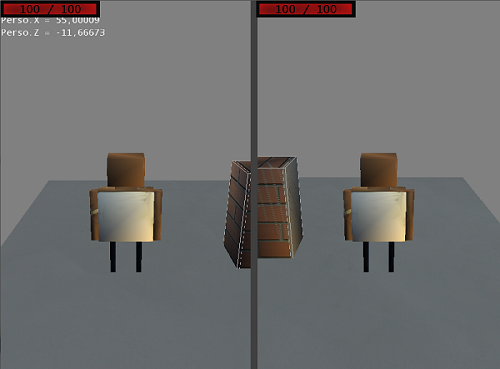
\includegraphics[scale=1]{Multijoueur.png}
\caption{Mode multijoueur}
\end{center}
\end{figure}

Chaque joueur a son propre personnage, sa propre barre de vie ainsi que sa propre camera. L'essentiel du mode multijoueur est donc fait, il ne manquera plus qu'à l'améliorer. Pour finir, j'ai créé un bouton multijoueur dans le menu d'accueil qui permet au joueur de choisir son mode de jeu : le mode solo ou le mode multijoueur.

Nous avions déjà un site web lors de la première soutenance, mais pour la deuxième nous avons décidé de modifier le design du site ainsi que la clarté du code comme Martin nous l'avait demandé. C'était à Anatole et moi-même de nous occuper de cette tâche. J'ai, avant tout, refait le design du site en faisant un croquis sur une feuille de papier. Puis j'ai relu une partie de notre code pour le modifier et l'amélioré.
\\
\\


Le travail fourni pour cette soutenance nous a vraiment fait avancé et progressé. Notre jeu ressemble de plus en plus à un véritable jeu vidéo.

\subsection{Tâches accomplies pour la troisième soutenance}
Pour la soutenance finale j'ai travaillé sur les mêmes tâches que celle de la deuxième soutenance excepté en ce qui concerne le réseau. Mis à part le réseau, notre travail pour cette soutenance est en fait un travail de finalisation et d'amélioration et non plus de création.

J'ai donc continué à m'occuper tout d'abord des graphismes pour avoir un joli rendu à l'écran. Les armes et certains éléments du décor étaient manquants. Cette partie-là ne m’a pas pris beaucoup de temps car je maitrisais assez bien Photoshop et Blender maintenant. Je me suis chargé de faire un plafond en reprenant le model du sol que nous avions mais en changeant la texture. Nous avons décidé de faire deux armes : un couteau assigné par défaut au personnage et un pistolet qu’il devra trouver et ramasser dans la prison pour pouvoir l’utiliser. Pour le pistolet et le couteau j’ai dû créer de nouveaux modèles avec le logiciel Blender et leur appliquer à chacun une texture, à l’aide de Photoshop, comme pour les décors précédents.

Cependant, pour que le personnage puisse tenir une arme (pistolet ou couteau) ce fut un peu plus compliqué. J’ai dû reprendre les modèles de nos personnages et les modifier avec l’aide de Louis pour faire en sorte qu’ils tiennent l’arme en question. Pour réaliser cette prouesse je me suis uniquement servi de Blender. J’ai effectué cette tâche en dernier car je devais avoir à ma disposition les modèles des deux armes. Au final, le décor de la prison est complètement fini et les personnages peuvent enfin disposer d’une arme.

Le mode multijoueur était pratiquement terminé dès la deuxième soutenance, mais je voulais l’améliorer en ajoutant un timer. C’est-à-dire une sorte de chronomètre qui indiquerait le temps que mettrais chaque joueur pour sortir de la prison. Le joueur qui sortirait de la prison le plus rapidement possible serait déclaré vainqueur. Pour cela il fallait que je trouve comment récupérer le temps entre deux points (point de départ et d’arrivée du personnage). Il existe sur XNA, une fonction qui permet justement d’obtenir ce que je voulais. Pour rendre le timer esthétique et améliorer la jouabilité j’ai décidé de l’afficher en haut des deux écrans scindés pour que les joueurs puissent à, tout moment, se rendre compte de leur avancée dans le jeu.

Le réseau fut la grande épreuve de la troisième soutenance et la tâche la plus compliquée également. Anatole et moi-même devions nous en occuper. Cependant, mis à part un TP réalisé au milieu de l’année nous ne connaissions strictement rien au réseau. Nous savions que pour que notre jeu fonctionne en réseau il allait falloir récupérer la position du personnage principal ainsi que celle des ennemis sur la carte pour chaque joueur et transmettre ces données à un serveur pour que chaque joueur reçoive les données des autres joueurs. Mais ce n’était pas fini, il fallait aussi récupérer les données des personnages et des ennemis (barre de vie et arme tenu). Nous connaissions donc le principe mais nous ne savions pas l’appliquer. La solution pour ce problème fut la recherche de tutoriel concernant le réseau. Nous avons trouvé des tutoriels très utiles sur MSDN, la librairie intégrée à tous les outils de développement de Microsoft, ainsi que sur Youtube. Avec l’aide de ces tutoriels et du TP réalisé au cours de l’année le réseau fut beaucoup plus compréhensible pour nous, il nous a cependant pris un peu plus de deux journées pour être entièrement fonctionnel.

Le site web a subi de nombreuses améliorations pour cette soutenance finale notamment la possibilité de choisir la langue (français ou anglais). Un logiciel nommé Dreamweaver permet de gérer beaucoup plus facilement la mise en page. Ce logiciel affiche d’un côté le code HTML et CSS et de l’autre côté le rendu. Il offre la possibilité de modifier directement le rendu sans avoir à retaper des lignes de codes. Anatole et moi-même nous sommes donc servis de ce logiciel pour améliorer le design et la mise en page de notre site plus rapidement. De plus, la clarté et la compréhension du code ont été grandement améliorées.

\subsection{Problèmes rencontrés lors du projet}
Ce projet est un projet que nous avons choisi et qui nous tenais à cœur, mais cela ne signifie pas que nous n’avons rencontré aucuns problèmes lors de son déroulement. Lors de la réalisation de ce projet j'ai dû faire face à plusieurs obstacles. L'obstacle le plus difficile et le plus récurrent fût celui des connaissances et de l'expérience. L'informatique étant nouveau pour moi, sous cet angle, je ne possédais pas les éléments nécessaires pour la réalisation d'un tel projet. J'ai donc dû effectuer de nombreuses recherches ce qui demande beaucoup de temps et ce qui n'est pas toujours évident avec les cours, les examens... Le début du projet fût la partie la plus difficile, je ne savais pas par où commencer, tout me semblais extrêmement compliqué. Heureusement, Louis et Anatole possédaient déjà un bon niveau en informatique et en programmation, j'ai donc pu débuter le projet en partie grâce à eux. Leur aide me permis de débuter le projet, j'ai pu me débrouiller tout seul par la suite.

Le temps et l'organisation furent également un problème qu'il a fallu gérer rapidement. En effet, comme je vous l'ai dit précédemment, avec les cours, les examens et les activités extra-scolaires de chacun le temps manque. De ce fait, bien préparer les différentes soutenances en respectant notre programme figurant dans le cahier des charges était un véritable défi. Louis, Anatole et moi étions dans la même classe mais Lenny n'étant pas avec nous ce ne fût pas toujours facile de s'organiser pour travailler en dehors des semaines réservées pour la préparation des soutenances. Heureusement nous étions un groupe solidaire et soudé, nous ne nous sommes pas découragés et le travail a fini par payer.

L'ambition fût également un de nos problèmes. Nous avions chacun une image précise de notre jeu en tête, un jeu parfait. Or, notre jeu ne pouvait pas ressembler à ce que nous imaginons. Il a parfois fallu nous raisonner sur certaines choses que nous voulions faire mais qui n'étaient pas possible, faute de temps et de connaissances. Il a fallu que nous nous imposions des limites pour veiller à respecter notre programme et nos objectifs.

\subsection{Conclusion personnel}
Le projet Evasion fût une expérience incroyable. Durant la réalisation de notre projet j'ai pu apprendre énormément et sur différents plans. D'une part d'un côté informatique, mes connaissances en programmation se sont véritablement améliorées. J'ai appris que la maîtrise de l'informatique était impossible sans un travail important de recherche. De plus j'ai pu découvrir de nombreux logiciels qui peuvent être utiles dans la vie courante (Photoshop, Github). D'une autre part, le fait de travailler en groupe est une idée qui me plaît. Cela nous forme au travail en entreprise que nous aurons à effectuer plus tard. Nous développons grâce à cette expérience un côté relationnel extrêmement important qui est indispensable. J'ai pu constater lors de ce projet l'importance de l'organisation et de la communication dans un groupe. Sans cette cohésion, cette solidarité et les échanges que nous avons pu avoir, jamais notre projet aurait pu aboutir. Il y a certes des désaccords dans un groupe, mais le fait de communiquer et de s'exprimer, donner son avis permet d'avancer et de faire progresser le travail d'équipe et donc le projet.

Je peux donc dire que la réalisation de ce projet apporte une expérience indispensable pour nous, futur ingénieur, qu'il nous prépare aux situations auxquelles nous serons confrontés plus tard. Je suis content d'avoir participé à ce projet et encore plus de l'avoir vécu avec ce groupe.






\newpage

\section{Bibliographie}
\noindent
-HILAIRE Nicolas, \textit{Apprenez à développer en C\#}, Paris, Le livre du Zéro, 2012. 512p. \\
Livre qui explique les bases du C\#. 

\section{Webographie}
\subsection{Site Internet}
\noindent
- Développez.net. [En ligne]. Disponible sur : \underline{http://www.developpez.net/forums/} \\
Un forum pour les développeurs qui recense problèmes et solutions. \\
- MSDN. [En ligne]. Disponible sur :  \underline{http://msdn.microsoft.com/fr-FR/} \\
Librairie intégrée à tous les outils de développement de Microsoft. \\
- Open Classroom ou Le site du Zéro. [En ligne]. Disponible sur : \underline{http://fr.openclassrooms.com/} \\
Site proposant de nombreux tutoriels pour débutant concernant différent domaine de l'informatique. \\
- Find sounds. [En ligne]. Disponiblle sur :  \underline{http://www.findsounds.com/} \\
Ce site nous a permis de récupérer des sons d'ambiances pour notre jeu vidéo.\\
- Dotnet. [En ligne]. Disponible sur :  \underline{http://www.dotnet-france.com/} \\
Site qui contient une bibliothèque .NET qui nous a servi pour le réseau. 
\subsection{Vidéos Youtube}
\noindent
-  \underline{http://www.youtube.com/watch?v=XkpZLzT5OV4} \\
Tutoriel pour créer une caméra à la première personne. \\
-  \underline{http://www.youtube.com/watch?v=WckzgfieBXo} \\
Vidéo expliquant l'utilisation de la classe Viewport nécessaire pour le mode multijoueur. \\
-  \underline{http://www.youtube.com/watch?v=JdSNgYaY9Y0} \\
Video expliquant les bases du reseau en C\# avec XNA. 

\newpage

\thispagestyle{empty}
\pagestyle{fancyplain} \chead{}\lhead{\textit{Les Professionnels}} \rhead{\emph{\textit{Evasion}}}
\listoffigures

\end{document}
